\documentclass{article}
\usepackage[utf8]{inputenc}
\usepackage{titling}
\usepackage{geometry}
\usepackage{graphicx}
\usepackage{siunitx}
\usepackage{amsmath}

\geometry{
  left=1.5cm,
  right=1.5cm,
  top=2.5cm,
  bottom=2.5cm,
  bindingoffset=5mm}
  
  
\begin{document}
\begin{titlepage}
	\centering
	
\includegraphics[scale=0.1]{KIT.png} \par\vspace{4cm}
	{\scshape\LARGE Karlsruher institute of technology \par}
	\vspace{1cm}
	{\scshape\Large Betriebswirtschaftslehre\par}
	\vspace{1.5cm}
	{\huge\bfseries Rechnungswesen\par}
	\vspace{2cm}
	{\Large\itshape Fabian Pöhler\par}
	\vfill
	
	\vfill

% Bottom of the page
	{\large \today\par}
\end{titlepage}
\newpage
\tableofcontents
\newpage

\section{Grundlagen des Rechnungswesen}

\subsection{Realisationsprinzip}

Ab wann sollen Transaktionen als realisiert gelten. Hierzu muss die Transaktion komplettiert sein. Dies ist der Fall, wenn:
\begin{itemize}
\item eine hohe Sicherheit besteht, dass das Unternehmen ökonomisch
von der Transaktion profitiert,\\
\item die Messung der Erträge und verbundenen Aufwendungen zuverlässig
erfolgen kann und\\
\item das Unternehmen mit der Transaktion verbundene Risiken und
Nutzungsvorteile auf den Transaktionspartner transferiert hat.
\end{itemize}
\begin{center}
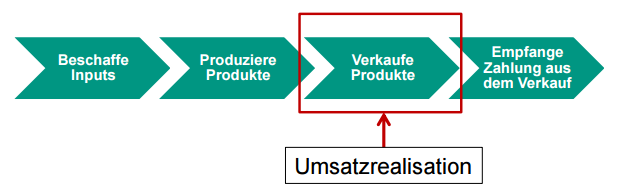
\includegraphics[scale=.5]{umsatzrealisation.png}
\end{center}

\subsection{Matching principle}

Wann sollen Aufwendungen in die Gewinnberechnung einfließen? \\
Das Matching Principle sieht vor, dass Aufwendungen in die
Gewinnberechnung für diejenige Periode einfließen, in der die Erträge, die
diese verursachen, als realisiert gelten.
So fließen die Erträge und ihre verursachten Aufwendungen in den Gewinn
derselben Periode ein.
Es ist dabei nicht entscheidend, dass in dieser Periode auch eine
aufwandsverbundene Auszahlung erfolgt.
Beispiel: Aufwendungen für die Produktion von Produkten fließen dann in die
Gewinnberechnung ein, wenn die Produkte verkauft werden und der Umsatz
realisiert wird.

\section{Jahresabschluss und Geschäftsbericht}

Es gibt zwei Verfahren der GuV-Aufstellung:

\subsection{Umsatzkostenverfahren}

Umsatzerlöse - Umsatzaufwand = Brutto-Ergebnis vom Umsatz \\
+ Sonstige Erträge - Vertriebsmittel - Allgemeiner Verwaltungsaufwand - Sonstige Aufwendungen = Ergebnis der betrieblichen Tätigkeit \\
+ Finanzerträge - Finanzierungsaufwendungen = Periodenergebnis vor Steuern\\
 - Ertragssteueraufwand = Periodengewinn/verlust 

\subsection{Gesamtkostenverfahren}

Umsatzerlöse + Sonstige Erträge +/- Bestandveränderungen fertiger und unfertiger Erzeugnisse - Materialaufwand - Personalaufwand - Planmäßige Abschreibungen - Sonstige Aufwendungen = Ergebnis der betrieblichen Tätigkeit \\
+ Finanzerträge - Finanzierungsaufwendungen = Periodenergebnis vor Steuern\\
 - Ertragssteueraufwand = Periodengewinn/verlust 

\subsection{Kapitalflussrechnung}

Cash Flow aus laufender Geschäftstätigkeit
+ Cash Flow aus der Investitionstätigkeit
+ Cash Flow aus der Finanzierungstätigkeit
= Zahlungswirksame Veränderung des Finanzmittelbestandes

\subsubsection{Cashflow aus laufender Geschäftstätigkeit}

\textbf{Direkte Methode:}\\
Cash Flow aus laufender Geschäftstätigkeit = Operative Einzahlungen - Operative Auszahlungen \\
\textbf{Indirekte Methode:}\\
Cash Flow aus laufender Geschäftstätigkeit = \\
Periodenergebnis vor außerordentlichen Posten\\
+/- Abschreibungen/Zuschreibungen auf Gegenstände des Anlagevermögens\\
+/- Zunahme/Abnahme der Rückstellungen\\
+/- Sonstige zahlungsunwirksame Aufwendungen/Erträge\\
-/+ Gewinn/Verlust aus dem Abgang von Gegenstanden des Anlagevermögens\\
-/+ Zunahme/Abnahme der Vorräte, der Forderungen aus Lieferungen und Leistungen sowie anderer Aktiva, die nicht der Investitions- oder Finanzierungstätigkeiten zuzuordnen sind \\
+/- Zunahme/Abnahme der Verbindlichkeiten aus Lieferungen und Leistungen sowie anderer Passiva, die nicht der Investitions- oder Finanzierungstätigkeiten zuzuordnen sind\\
+/- Ein- und Auszahlungen aus außerordentlichen Posten\\

\section{Bilanzierung}

\subsection{Fair value}

Als fair value wir derjederjenige Preis bezeichnet, den der Vermögenswert beim jetzigen Verkauf erbringen würde.
Der bestmögliche fair value ist der Marktpreis einess/r vergleichbaren Transaktion.
\section{Operationale Effizientanalyse}

\subsection{Working Capital Requirement}

$WCR = Operative Vermoegenswerte - Operative Verbindlichkeiten $ 

mit $ Operative Vermoegenswerte = Forderungen aus LL + Vorraete + gezahlte Anzahlungen + Aktive Rechnungsabgrenzeungsposten$

und  Operative Verbindlichkeiten = Verbindlichkeiten aus LL + Passive Rechnungsabgrenzungposten + erhaltlene Anzahlungen + Sonstige Verbindlichkeiten für das operative Geschaeft 

\subsection{Kennzahlen der Liquidität}
\subsubsection{Net long-term Financing}
$NLF = langfristige Schulden + EK + langfristige Vermoegenswerte$

\subsubsection{Net short-term Financing}
$NSF = kurzfristige nichtoperative Schulden - Zahlungsmittel $

\subsubsection{Liquidity Ratio}
$LR = \frac{NLF}{WCR}$

\subsubsection{Auswirkungen der Branche auf das WC}

$WCR-to-sales Ratio = \frac{WCR}{Umsatz}$


\subsubsection{Umschlagsdauer und Häufigkeit}

$Umschlagshaeufigkeit des Vorrats = \frac{Umsatzkosten}{durchschnittlicher Bestand}$

$Umschlagsdauer = \frac{365}{Umschlagshaeufigkeit}$

$Kundenziel = \frac{Forderungen aus L\&L * 365}{Umsatz} $

$Lieferantenziel = \frac{Verbindlichkeiten aus L\&L * 365}{Endbestand Vorraete - Anfangsbestand + Umsatzkosten - Fertigungskosten}$

\subsection{Traditionelle Liquiditätsmaße}
$NWC = UV - kurzf. Schulden$

Liquidität 1. Grades: $ L1 = \frac{Zahlungsmittel}{kurzf. Schulden}$

Liquidität 2. Grades: $ L2 = \frac{Zahlungsmittel + Forderungen aus L\&L}{kurzf. Schulden}$

Liquidität 3. Grades: $ L3 = \frac{Zahlungsmittel + Forderungen aus L\&L + Vorraete}{kurzf. Schulden}$

 



\section{Bilanzanalyse}
\subsection{Differenzierungsmöglichkeiten}
\subsubsection{Absolute Kennzahlen}

EAT, EBT, EBIT, EBITA, EBITDA

\subsubsection{Relative Kennzahlen}

Umsatzrentabilität:   $ ROS =  \frac{Jahresueberschuss + Zinsaufwand + Steuern}{Umsatz} = \frac{EBIT}{Umsatz} $ 

Eigenkapitalrentabilität:  $ ROE = \frac{Jahresueberschuss}{Umsatz} $

$ ROIC = \frac{EBIT}{Investiertes Kapital} = \frac{EBIT}{Capital Employed} = \frac{EBIT}{Umsatz}*\frac{Umsatz}{Investiertes Kapital} $

mit Investiertem Kapital = $ Zahlungsmittel + WCR + langfr. Vermoegenswerte + nicht-operative kurzf. Vermoegenswerte$

und Capital Employed = $ kurzf. nicht-operative Schulden + langf. Schulden + Eigenkapital $

$ ROBA = \frac{EBT+Zinsauaufwand}{WCR+langf. Vermoegenswerte} $

$ROTA = \frac{EBIT}{Alle Vermoegenswerte} $

$Financial Cost Ratio = \frac{EBT}{EBIT} $

$Financial Structure Ratio = \frac{Investiertes Kapital}{Eigenkapital} $

$Financial Leverage Multiplier = Financial Cost Ratio x Financial Structure Ratio$

$Tag-Effect Ratio = \frac{Jahresueberschuss}{EBT} = 1 - effektiver Steuersatz $ 
 
\subsubsection{Marktwertbasierte Kennzahlen}

$Gewinn je Aktie = \frac{Jahresueberschuss}{Durchschnittliche Anzahl der Aktien}$

$KGV = \frac{Preis je Aktie}{Gewinn je Aktie}$

$Market-to-Book Ratio = \frac{Preis je Aktie}{Buchwert des Eigenkapitals je Aktie}$ 

\subsubsection{EBIT-Multiple}

$EBIT-Multiple = \frac{Enterprise Value}{EBIT} = \frac{Marktwert der EK + Finanzschulden - Zahlungsmittel}
{EBIT}$

$ Enterprise Value = \frac{EBIT}{i}$

Wachstumsrate $g = i - \frac{EBIT}{Enterprise Value} = i - \frac{1}{EBIT-Multiple}$


\subsubsection{Monetäre und nicht-monetäre Kennzahlen}
Reantabilitäts oder Erfolgskennzahlen oder Markt und Kundenkennzahlen


\section{Wertorientierte Unternehmensführung}

\subsection{Eigenkapitalkosten}
Die Eigenkapitalkosten berechen sich mit dem CAPM:

$ k_e = r + ( \mu - r ) * \beta $

wobei r die Rendite der sicheren Anlage, $ \mu $ die erwartete Marktportfoliorendite und  $ \beta $ das Beta der Aktie ist.

\subsection{Kapitalkosten}
Die Kapitalkosten WACC bestimmen sich wie folgt:

$WACC = \frac{EK}{FK + EK} * k_{e} + \frac{FK}{EK + FK} * k_{f} * (1-s)$

wobei s der Marginale Steueratz ist.

\subsection{Economic Value Added}

$EVA =  NOPAT - WACC * CapitalEmployed $

\subsubsection{Gewinn vor Kapitalkosten}

$NOPAT = Jahresueberschuss + Zinsaufwand * (1 - s)$


\section{Budgetierung}

\subsection{Budgetierung}
\begin{center}
\item Untersuchung der Unternehmensumwelt und des Unternehmens auf
Veränderungen.
\item Prognose von budgetrelevanten Faktoren in der nächsten Periode auf Basis
von Informationen aus der Vorperiode.
\item Festlegung von Zielen für die Budgets des Gesamtunternehmens und
wichtiger Unternehmensbereiche unter Berücksichtigung der Informationen
aus Schritt 1 und 2 und der Budgetabweichung und deren Ursachen aus der
Vorperiode.
\item Erstellung eines Gesamtbudget-Vorschlags durch die Unternehmensführung
und Ableitung von Budgetentwürfen für die einzelnen Bereiche.
\item Planung der Einzelbudgets durch die dezentralen Planungseinheiten.
\item Einreichen der dezentral erstellten Budgetanträge an die genehmigenden
Instanzen. 
\item Prüfung der Budgetanträge bezüglich formeller und matrieller Aspekte.
\item Abgleich der top-down mit den bottom-up bestimmten Werten.
\item Koordination der Teilpläne und Zusammenfassung zu einer Gesamtberichterstattung
\item Genehmigung aller Budgets durch die Unternehmensleitung.

\end{center}

\subsection{Benchmarking}
Benchmarking als Ansatz des Lernens von Anderen zur Lösung eigener
Probleme. Es wird als Instrument der taktischen Planung klassifiziert.
\subsubsection{Ziele des Benchmarking} 
Identifikation von marktorientierten Zielvorgaben zur Bewältigung von
eingefahrenen Denkweisen und Selbstzufriedenheit.
Identifikation und Verständnis von besseren Wegen zur Erreichung dieser
Ziele und zum Aufbrechen ineffizienter und verkrusteter Strukturen.
\subsubsection{Erfolgsfaktoren eines Benchmarkingprojektes}
Sorgfältige Vorbereitung bezüglich Umfang und Ziele.
Hierarchieübergreifende Unterstützung durch Top-Management und
Process Owners.
Aussagefähigkeit und Definitionsgenauigkeit der Vergleichskennzahlen.
Sicherstellung der Vergleichbarkeit und Lernpotenzials bei der Selektion
der Vergleichspartner.
Sicherstellung von Veränderungsbereitschaft und Machbarkeit im
Implementierungsprozess.


\end{document}
